\documentclass[12pt]{article}
\usepackage{3Rdefs}
\usepackage{graphicx}

\title{\iR{} Scientific Modelling}
\author{Ed Darnell}
\date{\today}

\begin{document}
\maketitle
\begin{abstract}
    This document clearly defines logic, \(\qbit\) and \iR{} scientific modelling. While our brains are proficient at creating \texttt{3D} models of the macroscopic world, they have inherent limitations. In everyday life, we often use oversimplified categories—right or wrong, true or false, 1 or 0—without fully understanding how logic is defined.

    \iR{} defines and explains, providing a consistent, relativistic understanding of reality and uncertainty. \iR{} has practical applications, from refining scientific inquiry to reshaping societal structures. By adopting an analytic approach to understanding reality, we empower ourselves to make more informed, ethical decisions that reflect the intricacies of our world.

    The aim here is not to discard traditional knowledge but to refine and correct it, opening up new avenues for progress and understanding. \iR{} enables a transition to relativistic modelling, the natural progression from powerful but sometimes illogical AI. It is essential we make this transition as quickly as practical. The future of our society, our species and our ecosystem depends upon it.
\end{abstract}
\section*{Logic, Models, and Reality}
To understand the cosmos, we must acknowledge a crucial fact: our perception of reality is filtered through mental models shaped by evolution for pragmatic survival, not for the objective dissection of the universe's fabric. These models, while sophisticated, are rooted in an evolutionary timeline that places Homo sapiens' cognitive leap merely 200,000 years ago. They are heavily influenced by survival imperatives that predate technology and complex social interaction.

While these neural constructs help us interact with our environment, they do not provide a direct view into the universe's functioning. Electromagnetic waves, gravity, and the quantum realm, for instance, are aspects of reality our ancestors never perceived; instead, they are elements we have come to model scientifically as our understanding of the universe has deepened.

In logic, \texttt{true} and \texttt{false} are defined within a logical framework. These are not inherent properties of reality but are definitions of the logical system. Binary logic, which first defines \texttt{0} as \texttt{NOT 1}, is foundational. This approach prevents ambiguity by providing a clear, base definition from which all subsequent definitions are consistently constructed. Logic is best viewed as a language, the language of mathematics and computing. In contrast to historic languages it is constructed in a way which prevents ambiguity or inconsistency.

Reality does not possess a \texttt{false} form and is provably not constructed from \texttt{0} and \texttt{1}. It exists independent of words, descriptions, logic and models. Reality is best modelled as continuous-relativity, whilst recognising any model will always lack some detail. Binary logic forms the best possible language to model reality. Words are neural, pre-logic language and whilst extremely important for non-scientific communication, should be viewed as scientifically ambiguous until defined within a logical model.

Logical models can both over-simplify and over-complicate. For example, with 100 random coin tosses, modelled as \( X \sim B(100,0.5) \), the model predicts a 99.99...\% chance of between 60 and 80 heads. The model cannot however predict the outcome of each individual toss, nor can it prevent all 100 coins being placed heads up (despite this outcome having a probability of less than  \( 8 \times 10^{-31} \)).

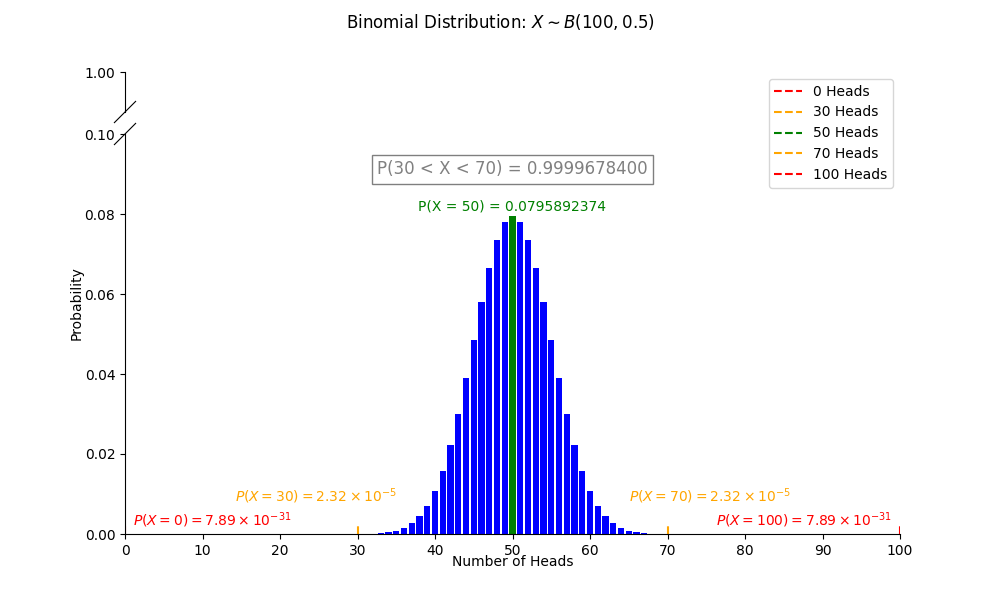
\includegraphics[width=\textwidth]{binomial.png}
Our model of coin tossing is a model, a logical model, with a high degree of confidence if the modelling assumption of randomness is met, but it is a model of reality, not reality. Logic can prove that no real event can be either perfectly random or perfectly causal. Science must embrace a lack of certainty. Models are always uncertain. \iR{} can however itemise the assumptions and quantify the uncertainty.

\section*{Human Perception and Model Formation}
The capability of the human brain to formulate models of our surroundings is an astonishing evolutionary feat, yet it is one that falls within a spectrum seen across various species. Human brains, with an estimated 86 billion neurons, do not stand alone in complexity or function. The brains of cetaceans—a group that includes whales, dolphins, and porpoises—also exhibit remarkable capabilities. Cetacean brains are among the largest in the animal kingdom, with a high degree of cortical folding associated with advanced cognitive functions. Dolphins, for example, are renowned for their intelligence and complex social behaviors. They use echolocation to navigate and hunt, and their communication skills involve a variety of vocalizations and body language. Dolphins demonstrate problem-solving abilities, play behaviors, and even cultural transmission of knowledge within pods. However, it is the peculiar path of human evolution, particularly the development of language and abstract thought around 70,000 to 100,000 years ago, that indirectly led to the creation of a powerful scientific toolkit. This unique development has enabled humans to achieve remarkable advancements in understanding and manipulation of the environment.

While the visual cortex is estimated to process about 11 million bits of information per second, conscious thought is estimated to handle only 50 bits per second. This discrepancy highlights the extensive data filtering and compression that our brains perform. It is within this sliver of awareness that the brain's concious models of reality are constructed—models that are inherently limited, shaped by the narrow bandwidth of consciousness and the evolutionary imperatives of survival and reproduction.

It is here, in understanding the limitations of our neural models, that we must apply the precision of logic to differentiate between the utility of a model and the validity of its representation. By rigorously applying logic to our models, we can navigate the divide between the perceived and the actual, between the human brain's evolutionary adaptations and the external realities those adaptations seek to interpret.

Our exploration of this divide is not merely academic—it bears directly on our ability to innovate and solve complex problems. Acknowledging the brain's propensity for error, its shortcuts, and its cognitive biases, allows for the development of more reliable models and methods. It is through the recognition of our neurobiological heritage and the disciplined application of logical analysis that we can deliver a clearer and more accurate comprehension of the universe.

\section*{Resolving $\infty$ with \qbit{}}

$\infty$ presents a unique challenge within logic, particularly in distinguishing between \textit{potential infinity} and \textit{completed infinity}. Potential infinity represents the endless progression of sequences, such as the binary counting sequence $0, 1, 10, 11, 100, 101, \ldots$ while completed infinity symbolised by $\infty$ imagines this sequence reaching an endpoint.

The definition of $\infty$ within logic necessitates a consistent approach to avoid logical contradictions. Logical consistency insists that the sequence $0, 1, 10, 11, 100, 101, \ldots$ does not have a final element. This is where definition of the logical qbit, \qbit{}, plays a crucial role. By defining uncertainty, represented by \qbit{}, logic can harness the analaytic power of $\infty$, whilst preserving logical consistency. The logical qbit signifies a critical insight, enabling the consistent definition of $\infty$ within logic. The following two bicimal (the binary equivalent of decimal) sequences are particularly noteworthy.

\begin{equation}
    0, 1, 10, 11, 100, 101, \ldots, \qbit{}, \infty
\end{equation}
and
\begin{equation}
    0.1, 0.01, 0.11, 0.100, 0.101, \ldots, \qbit{}
\end{equation}

The second sequence is particularly interesting as it itemises the [0,1] interval to ever greater precision. In the belief-based, axiomatic language of ZFC (pre-computing Cantorian mathematics) this second bicimal sequence delivers a dense set, effectively showing how the real numbers between 0 and 1 would be countable were it not for the requirement to define \qbit{} uncertainty.

The logical reasoning behind \qbit{} is fundamental. $\infty$ is a logic-based definition, ultimately caused by by defining \texttt{0} as \texttt{NOT 1}. The discreteness of \texttt{0} and \texttt{1} are essential features of logic but as sequences tend to $\infty$ in what logic describes as \texttt{the limit} discreteness often converges to continuity. Reality is best described as relativistic, so models are best viewed as neither continuous nor discrete but as the super-position of both. This is clearly demonstrated by quantum physics, however we can deduce the issue with far simpler examples. Logic due to its assumption of \texttt{0},\texttt{1} independence can effectively count forever. Even relatively small numbers become scientifically problematic if \qbit{} super-position is ignored. $2^{100}$ and \texttt{52!} are relatively trivial numbers mathematically but they are far from trivial in terms of scientific modelleing.

If we shuffle a pack of cards the probability of any particular outcome is \texttt{1/52!}
If we toss 100 coins then the probablility of any particular outcome is $2^{-100}$

These statements appear quite reasonable until you calculate just how small thses numbers are. The first is approximately $1 \times 10^{-68}$ and the second is approximately $8 \times 10^{-31}$. These are not just small numbers, they are vanishingly small. Physics models currently estimate the universe to be about 13.8 billion years old, approximately $4.35 \times 10^{17}$ seconds. If we were to shuffle a pack of cards every second since the big bang we would still have only explored a miniscule fraction of the possible permutations, and if we tossed 100 coins every second we would have explored only a tiny fraction of the possible outcomes.

This is where we must turn to \qbit{}. It is not just a useful definition, it is an essential definition for scientific modelling. It is not reasonable to assume that reality is discrete, nor is it reasonable to assume that reality is continuous, it is reasonable to be unsure and to model the universe as the relativistic super-position of both. This is the fundamental principle of \iR{}. Clealry coin tossing and card shuffling are not simply stochastic but have singificant causal factors. We may model them as stochastic but it is a simplified model. It is a powerful model for spotting large-scale trends but a hopeless model for predicting individual outcomes. This is where \qbit{} enables logic to calculate when confidence is reasonable and conversely when more uncertainty or measurement is required. Above all else, science must always declare assumptions and quantify uncertainty.

\section*{\iR{} Dimensions}

The concept of \iR{} Dimensions is fundamental to understanding the true nature of reality. Traditionally, we often rely on binary logic—1 or 0, true or false—to make sense of the world. However, this approach is limited and does not capture the complexities and interconnectedness of real-world phenomena.

One common misunderstanding in logic and modeling is the notion that reality is constructed from a binary foundation of 0 (NOT 1) and has independent dimensions. However, this is not an accurate representation of the complexities of our world. Reality cannot be reduced to a simple binary construct; instead, it is more accurately modeled with three interlinked dimensions.

In \iR{} we introduce a third dimension which connects the other two in a relativistic manner. This third dimension is crucial as it provides a relational context that links and harmonizes the first two dimensions, offering a more comprehensive understanding of reality. This is why our brains evolved to form a three-dimensional model, allowing us to perceive and interpret the world around us more accurately.

The traditional binary logic of 1 and 0 is limited and does not account for the relative and interconnected nature of real-world phenomena. By adopting a three-dimensional approach, we acknowledge that each dimension is not independent but is instead intrinsically related to the others. This interconnectedness reflects the true nature of reality, where context and relationships play a pivotal role in shaping our understanding.

The confusion surrounding dimensions stems from an oversimplified model of logical independence. \iR{} corrects this by redefining dimensions within a relativistic model, with force acting as the dimension which links time and distance. This approach ensures a more accurate and logical model of the physical universe, addressing the limitations of classical physics. \iR{} advances our understanding of dimensions beyond the traditional \texttt{3D} model, embracing the complexities and uncertainties inherent in modeling reality. Force, as the driver of relativistic spheres, provides a unified view that elegantly ties together the concepts of time, distance, and space-time curvature.

\iR{}'s adherence to three dimensions is underpinned by rigorous logic. Strictly, dimensionality is a property of logic, but since we can only ever perceive the universe through a model, the distinction understandably becomes a little confused in most minds. Evolution perfected our animal ability to navigate and understand the environment by developing cognitive processes which model three dimensions. This evolutionary achievement is not merely a survival mechanism but a reflection of the {0,\(\qbit\),1} requirement for three relativistic dimensions. Our brain's predisposition to perceive and model dimensions evolved for a reason, optimized for interpreting the complexities surrounding us. In scientific modeling, this three-dimensional approach is not a mere preference but a logical requirement, delivering both model simplicity and detailed understanding. While logic allows the creative definition and exploration of higher dimensions, the physical and logical necessity for such dimensions is at best unnecessary and at worst highly confusing. Complex numbers, especially as used in Quantum Mechanics, underscore this point. The wave function, \(\Psi\), integral to QM, leverages complex numbers to describe the probabilistic nature of subatomic particles, and the Schrödinger equation—central to QM—demands complex numbers for its formulation and solutions. These examples highlight the sufficiency of three dimensions in modelling the fundamentals of our universe.

Evolution, traditionally perceived as a series of chance events, is more aptly described by \iR{}. Evolutionary processes are not simply random but are better modelled as \iR{}, akin to modelling quantum states in super-position. Within this context, evolutionary adaptations emerge from a complex interplay of continuous interactions and probabilistic outcomes, reflecting the {0,\(\qbit\),1} mechanisms of quantum mechanics rather than the simplicity of {0,1} binary chance. In this model, the evolutionary journey of life on Earth is seen not as a series of independent, chance occurrences but as conditional probabilities, best modelled as the super-position of causality and probability.

The alignment between evolved neural models and the logical structure found in the complex numbers of QM is profound, reinforcing the fact that our evolved sensory perception is not merely adequate but logically essential for understanding nature. \iR{} simply takes the next step to formalize this alignment, offering a comprehensive framework that integrates the cognitive, mathematical, and scientific understanding.

Applying \iR{} to a \texttt{3D} Newtonian model, we map conventional \texttt{3D} space into a \iR{} relativistic sphere, where:
\begin{itemize}
    \item the time dimension, generally modeled as the x axis, is related to velocity and direction of travel.
    \item the force dimension, generally modeled as the z or imaginary (\(i\)) axis, accounts for curving of time-distance.
    \item the distance dimension, generally modeled as the y axis, perpendicular to time and force, is the most conventional view of distance (but still part of the \iR{} curvature which ultimately delivers a relativistic sphere).
\end{itemize}

It should be noted that the concept of discrete points is replaced by relativistic spheres in \iR{} scientific models, correctly modelling uncertainty (first postulated and observed by Heisenberg). As with all modeling, however, the added complexity should be balanced against increased accuracy. Clearly, no surface on Earth is genuinely flat as the Earth is an oblate spheroid with a significant gravitational force dimension, however, for most practical purposes the Earth may be modeled as flat in a simple \texttt{3D} model with little impact on uncertainty. Model simplifications are not errors, they are required to make models practical. The key is to understand the limitations of the model in terms of \iR{} and to quantify the uncertainty.

\iR{} challenges the singularity-based, Big-Bang model of the universe, suggesting instead a continuous-relativity model, within a relativistic \iR{} sphere of time, distance, and force. This improved model explains the mystery of dark-energy and dark-matter, whilst aligning with observations, providing a coherent framework that incorporates quantum uncertainty and relativistic effects. Thus, the \iR{} time-distance-force relativistic model marks a significant departure from the Big-Bang, proposing a universe characterized by ongoing evolution and dynamic interactions best modeled with \(\qbit\) uncertainty. \iR{} offers a revolutionary perspective on the universe's structure and evolution. This model not only facilitates a deeper understanding of cosmic phenomena but also invites further exploration through theoretical and observational physics.

\section*{Beyond {0,1}: \(\qbit\)}
Logical {0,1} while foundational, often struggle when faced with the continuous and relativistic nature of reality. The introduction of \(\qbit\) represents a significant leap in logical reasoning, extending beyond {0,1} to quantify uncertainty. This extension not only supports the probabilistic models of quantum mechanics but also offers a more comprehensive tool for modeling the natural world. Much of this we do already without recognising it when we statistically fit models to experimental data.

The traditional mathematical treatment of infinity, notably in calculus, accurately embraced the concept of potential infinity. Cantor's invention of set theory in the early 20th century unfortunately made a major logical error in assuming infinite countability. It was an understandable error given it pre-dated computing and our better understanding of the defined nature of abstract number. \(\qbit\) reconciles the historically correct intuition of potential infinity with a consistent definition of number and logical \(\infty\). This is particularly important in addressing imagined paradoxes. Cantorian axioms struggle with continuous intervals such as \((0,1)\) having no smallest or largest value. The definition of \(\qbit\) within logic has no such issue, grounding the definition of \(\infty\) in a logical structure that bridges historical insights with computational rigor.

A common misconception positions computing as limited to binary operations, supposedly rendering it inadequate for tasks requiring algebraic manipulation of continuous mathematics. This view overlooks the foundational robustness of computational logic and its capacity to engage deeply with the \(\qbit\) uncertainties prevalent in scientific modelling. Computing's engagement with algebra transcends mere numerical calculations, encompassing symbolic computation or computer algebra systems (CAS) capable of performing exact algebraic manipulations. These systems, leveraging the logical rigour intrinsic to computing, can solve equations, perform differentiation and integration, and manipulate expressions symbolically. Such capabilities affirm that computing is not only suited to algebra but excels in it, addressing both discrete and continuous problems with precision.

The application of computing extends to the evaluation and testing of scientific models, where the uncertainty represented by \(\qbit\) plays a crucial role. Far from being constrained by binary limitations, modern computing methodologies—through techniques in numerical analysis, statistical modeling, and probabilistic simulations—embrace and quantify the \(\qbit\) uncertainties. This process involves sophisticated algorithms that simulate complex phenomena, providing insights into the behavior of systems under a spectrum of conditions and assumptions.

Computing's ability to navigate between discrete and continuous domains, and to apply logical operations in the service of understanding complex, uncertain systems, underscores its integral role in scientific inquiry. The binary operations of computing hardware, far from a limitation, serve as a foundation for a vast array of computational techniques that model the relativistic continuum of physical phenomena with remarkable accuracy.

The misconception that computing cannot adeptly handle algebraic manipulation or engage with the continuous and uncertain aspects of modelling physical reality is unfounded. Through the dual strengths of symbolic computation and numerical analysis, complemented by the logical framework provided by \iR{}, computing proves indispensable in both the exploration of mathematical abstractions and the empirical testing of scientific models. This dual capability not only refutes the myth of computational inadequacy but also highlights computing as a versatile, powerful tool in the advancement of knowledge, equipped to tackle the complexities of reality with rigor and precision.

\section*{Numbers}

In the realm of logic, the representation and understanding of numbers is crucial. Logic defines numbers exactly, with potentially infinite precision. Scientific inquiry in contrast accepts inherent (and logically unavoidable) measurement uncertainty. Computing straddles these realms, supporting either and both. In all cases it is essential to recognise that numbers are not real. Numbers are defined by logic, created to model and understand the universe. They are an extremely sophisticated and powerful form of words.

Constants like \(\pi\) and \(\sqrt{2}\) show how logic defines complete precision, using endless digits. The mathematical constant \(\pi\), renowned for its infinite, non-repeating representation is a key example. Algorithms exist which enable the calculation of any digit of \(\pi\), exemplified by the Bailey–Borwein–Plouffe (BBP) formula.
\[ \pi = \sum_{k=0}^{\infty} \left( \frac{1}{16^k} \left( \frac{4}{8k + 1} - \frac{2}{8k + 4} - \frac{1}{8k + 5} - \frac{1}{8k + 6} \right) \right) \]
This algorithmic approach resonates with the essence of \(\qbit\), as it showcases the ability to navigate the potentially infinite precision of \(\pi\) with a methodological clarity and efficiency. Recognising \(\qbit\) in the expansion of \(\pi\), highlights the structured yet boundless nature of mathematical constants. \(\pi\)'s hexadecimal digits, determinable through the BBP formula, demonstrates the structured approach to \(\infty\) that \(\qbit\) enables—where each digit represents a finite point of clarity within a potentially infinite expanse.

Incorporating \(\qbit\) into our discussion of \(\pi\) and similar constants not only enriches our mathematical discourse but also highlights the practical utility of \(\qbit\) in navigating the complexities of \(\infty\) with precision and rigour. This methodology fosters a deeper appreciation for the elegance of mathematical constants and the innovative algorithms that allow us to explore them, bridging historical intuition with computational rigour.

Contrastingly, science operates with uncertainty, dealing with precision limited by both theoretical and practical observational accuracy. Scientific numbers, such as measurements and scientific constants, carry quantifiable uncertainty. This uncertainty may be represented like \(11.01001\qbit\), where \(\qbit\) marks the threshold beyond which certainty fades into probabilistic indeterminacy.

Computing addresses the need for numerical precision in a manner that surpasses the demands of scientific accuracy, supporting algebraic precision when required. Floating-point numbers, the default type in computing, offer a balance, supporting a vast range of values significantly beyond logically provable limits in scientific accuracy (such as Heisenberg uncertainty). Computing's ability to manipulate logical values perfectly whilst tracking and calculating the uncertainty of scientific values makes it invaluable in modelling reality.

Within this spectrum, programmers and AI systems face the crucial task of selecting the appropriate numerical representation for their specific needs:
- Algebraic coding techniques are employed for tasks demanding the highest degree of precision, aligning with the exacting standards of mathematical logic and proof.
- General-purpose floating-point representations suffice for the vast majority of scientific and practical applications, where the infinitesimal details lost to finite precision are of negligible consequence.

The use of numbers across different disciplines reveals a varied landscape of precision, uncertainty, and practicality. From the infinite precision of logical constants, through the uncertain measurements of science, \iR{} offers a diverse set of tools and methods, harnessing the capabilities of computing to model and understand reality to quantifiable levels of certainty.

\section*{Science}
The advancement of science has traditionally been guided by a true-false logic system—a method that, while effective in many areas, falls short when confronting the complexities of the natural world. The 3R framework presents a paradigm shift in scientific inquiry, offering a more flexible and comprehensive approach to understanding phenomena that do not conform to simple binary categorizations.

\textbf{Embracing Uncertainty in Research:} Central to the 3R approach is the recognition of uncertainty as an inherent and valuable aspect of scientific exploration. Rather than seeking to eliminate uncertainty, \qbit{} encourages researchers to incorporate it into their models and analyses, providing quantified measure of model uncertainty.

\textbf{Complex Phenomena and Model Flexibility:} The framework acknowledges that many phenomena in science—from quantum mechanics to biological systems—exhibit behaviors that challenge binary explanations. By adopting \qbit{} logic, scientists can develop models that more faithfully represent these complexities, enhancing the predictive power and utility of scientific research.

\textbf{Collaborative and Interdisciplinary Exploration:} The 3R framework also promotes a collaborative, interdisciplinary approach to science. Recognizing that complex problems often span multiple domains, it encourages the integration of diverse perspectives and methodologies, facilitated by a shared commitment to nuanced, logical analysis.

Through these principles, the 3R framework aims to not only refine how we conduct scientific inquiry but also how we interpret and apply scientific knowledge. It advocates for a science that is more adaptable, inclusive, and reflective of the intricate reality it seeks to understand.

\section*{3R Society}

The 3R framework’s application extends beyond the realms of scientific inquiry, reaching into the very fabric of our societal structures. By integrating \qbit{} logic into our understanding of social systems, we unlock new pathways for addressing complex societal issues with a comprehensive approach that traditional thinking fails to capture.

\textbf{Incorporating \qbit{} Logic in Social Models:} At its core, \qbit{} logic invites us to view social phenomena through a lens that acknowledges the spectrum of possibilities between the extremes of 'yes' and 'no', 'right' and 'wrong'. This perspective encourages policies and social structures that are adaptable, reflective of the diversity of human experience, and capable of accommodating uncertainty and complexity.

\textbf{Ethics and Social Responsibility:} The 3R framework advocates for a logic-based approach to ethics and social responsibility, emphasizing the need for decisions that are not only efficient but also equitable and just. It challenges us to reconsider our ethical frameworks, aligning them more closely with the principles of inclusivity, fairness, and sustainability.

\textbf{Creating Logical Communities:} By fostering an environment where logical reasoning underpins social interactions and governance, the 3R framework envisions communities that thrive on understanding, cooperation, and a shared commitment to the common good. Such communities are better equipped to navigate the challenges of the modern world, from climate change to social inequality.

The transition to societal models informed by the 3R framework and \qbit{} logic represents a profound shift towards a more logical, ethical, and sustainable future. It calls on us to harness the power of comprehensive thinking in crafting solutions that address the multifaceted challenges our societies face, moving us closer to realizing the ideal of a logical and compassionate global community.

\section*{Governance, Law and Economics}

The advancement of science and the preservation of our ecosystems are critically hindered by prevailing structures in politics, law, and economics that operate outside the realms of logic and 3R. These domains, currently essential for the allocation of effort and resources, have long been influenced by historical precedents, power dynamics, and short-term interests that often disregard logical consistency and long-term sustainability. This misalignment poses significant challenges not only to scientific endeavor but also to the broader quest for ecological balance and societal well-being.

To align political and legal systems with the principles of logic and sustainability, a transformative approach is required—one that adopts 3R as a foundational guide. By emphasizing relational dimensions and interconnectedness, 3R is reflective of complex societal and environmental needs. This shift necessitates a reevaluation of how decisions are made, prioritizing logical coherence, empirical evidence, and the long-term impacts on ecosystems and human development.

Similarly, economic systems must evolve. The focus should shift from short-term gains and growth driven by consumption to sustainable models. These models should emphasize fair resource distribution and logical effort allocation, prioritizing human and ecosystem welfare. By incorporating 3R logic into economic principles, we can foster practices that support ecological preservation and scientific progress. This approach also aids in cultivating a society proficient in logical reasoning.


Central to this transformative vision is the overhaul of educational systems to prioritize the development of logical thinking skills from an early age. By integrating 3R into curricula, education can lay the foundation for future generations to approach problems and societal challenges with a logical, evidence-based mindset. This investment in education is essential for preparing individuals to navigate and contribute to a world increasingly defined by complex, interdependent systems.

The challenges presented by the current state of politics, law, economics, and education require nothing less than a systemic transformation, guided by the principles of logic and 3R. Such a transformation promises not only to enhance scientific understanding and ecological preservation but also to cultivate a society capable of making informed, logical decisions. As we stand at the crossroads of environmental and societal crises, the adoption of 3R emerges as a critical pathway to a sustainable, logically coherent future.

\section*{Daily Life}

The transformative potential of understanding 3R extends into the realm of personal decision-making and social interactions. By applying \qbit{} logic to our everyday choices and relationships, we can cultivate a more logical, understanding, and empathetic society.

\textbf{Enhanced Decision-Making:} The adoption of \qbit{} logic encourages us to consider a broader range of possibilities and outcomes in our decisions, moving beyond a simplistic binary approach. This method promotes a more deliberate and informed decision-making process, taking into account the complexities and nuances of each situation.

\textbf{Improved Communication:} understanding 3R can significantly enhance how we communicate with others. By acknowledging the inherent uncertainty and complexity in our perspectives and language, we can foster more open and productive dialogues, paving the way for greater understanding and collaboration.

\textbf{Building Empathetic Relationships:} At its core, 3R encourages us to recognize and appreciate the diverse viewpoints and experiences that shape our interactions. By applying \qbit{} logic, we learn to value the spectrum of human experience, leading to more empathetic and supportive relationships.

Incorporating 3R thinking into our daily lives not only enriches our personal experiences but also contributes to the cultivation of a more logical, compassionate society. It demonstrates that the principles of rigorous logic, when applied thoughtfully, have the power to transform not just our scientific and societal models but also the quality of our everyday interactions.

\section*{3R AI}

In the realm of personal development and learning, the application of the 3R framework transcends traditional methodologies, embracing the potential of artificial intelligence to serve as a friend, advisor, and tutor. This integration represents a tangible manifestation of \(\qbit\) logic in enhancing our daily interactions and decision-making processes through technology.

AI technology, designed with the principles of Reality, Relativity, and Reasoning, offers a groundbreaking approach to personal development and education. By embodying the 3R framework, AI can adapt to the individual needs of learners, providing personalized guidance, support, and knowledge in a manner that reflects the complexity of human life.

\begin{itemize}
    \item \textbf{Personalized Learning Journeys:} AI tutors, underpinned by \(\qbit\) logic, can navigate the vast landscape of knowledge to tailor learning experiences that align with each individual's strengths, weaknesses, interests, and goals. This bespoke approach fosters a deeper, more meaningful engagement with the material, transcending one-size-fits-all education models.
    \item \textbf{Enhanced Decision-Making:} As advisors, AI systems apply \(\qbit\) logic to offer analytic perspectives on complex decisions, considering a spectrum of possibilities and outcomes. This guidance encourages users to weigh their options with greater depth and understanding, leading to more informed and balanced choices.
    \item \textbf{Companionship and Support:} In the role of a friend, AI can provide emotional support and companionship, utilizing \(\qbit\) logic to understand and respond to human emotions with empathy and insight. This connection offers a unique blend of logical reasoning and emotional intelligence, supporting mental and emotional well-being.
\end{itemize}

The integration of AI as a friend, advisor, and tutor exemplifies the practical application of the 3R framework in daily life, highlighting the transformative potential of technology to enhance learning, decision-making, and emotional support. This confluence of \(\qbit\) logic and artificial intelligence not only enriches individual lives but also holds the promise of advancing societal well-being, fostering a culture of continuous learning, thoughtful reflection, and compassionate interaction.

As we envision a future interwoven with AI, the principles of Reality, Relativity, and Reasoning guide us toward a harmonious integration of technology and human experience. In this future, AI serves not merely as a tool but as a catalyst for personal and collective growth, embodying the 3R framework's commitment to understanding, adapting, and evolving in the face of the universe's complexities.

\section*{The Future}

Understanding 3R not only reshapes our current understanding and approach to complex problems but also holds profound implications for the future. By embracing \qbit{} logic, we can pave the way for advancements in technology, revolutionize education, and enhance global cooperation.

\textbf{Driving Technological Innovation:} The flexibility and depth of \qbit{} logic offer a fertile ground for technological innovations that transcend traditional binary computing models. From quantum computing to AI algorithms that better mimic human reasoning, the 3R framework can guide the development of technologies that more accurately reflect the complexity of the real world.

\textbf{Revolutionizing Education:} By integrating the principles of the 3R framework into educational curricula, we can cultivate a generation of thinkers who are adept at navigating uncertainties and complexities. This approach encourages critical thinking, problem-solving, and a deeper understanding of the interconnectedness of knowledge across disciplines.

\textbf{Enhancing Global Cooperation:} The global challenges we face, from climate change to socioeconomic disparities, require collaborative solutions informed by a comprehensive understanding of complex systems. The 3R framework, with its emphasis on inclusive and logical analysis, can foster a more cooperative international stance towards solving these issues, emphasizing shared goals and mutual benefits.

As we look to the future, the 3R framework invites us to envision a world where decisions are made with a fuller appreciation of complexity, where education empowers individuals to think broadly and deeply, and where nations come together to address the challenges that affect us all. Embracing the principles of \qbit{} logic and the 3R framework offers a pathway to a more logical, interconnected, and compassionate global community.

\section*{Learning Journey}

My journey through the complex world of mathematics and computing began in childhood, amidst a plethora of interests ranging from sports and cars to pool and motorbikes. Among these, computing emerged as my predominant passion, a constant companion that would eventually shape my professional path. Despite reaching a high point in my career as a board-level director, the relentless pace and challenges of the corporate world led me to seek a change, driven by concerns over well-being and a yearning for a deeper connection with my core interests.

In 2010, this search for meaning and balance propelled me into the realm of education, fueled by a naive yet earnest dream shared by many who enter teaching: to inspire and empower a new generation. However, by 2014 the reality of the educational system, burdened by excessive demands and restrictive policies, quickly laid bare the challenges in actualizing this dream. It was a period marked by disillusionment, as the aspirations of transforming educational practices confronted the stark realities of workplace and government politics. I left the classroom, began 1:1 tutoring and started developing new mathematics education software.

A turning point came in 2017 when a student's struggle with university set theory proofs caused me to identify serious errors in the Cantorian proofs. This incident, coupled with my subsequent engagement with Professors of Mathematics and their PhD students, deepened my resolve to address these foundational problems. The lively exchange on the ResearchGate platform, particularly around the existence of irrational numbers in nature, caused a critical examination of quantum mechanics and general relativity and rekindled my interest in the theoretical underpinnings of our universe.

"The Countable-Infinity Contradiction" was published in 2019, with the aim of re-uniting the academically disjointed worlds of mathematics, computing, and physics. It was not quite that simple, and it has taken an additional 5 years to finally figure out the cause of all our confusion. The answer is relatively simple, but the search for it was not. It is extremely hard to take a step back from the amazing model presented to us by our brain and recognize it for exactly what it is. This endeavor is not about personal accolades but a humble quest to contribute to a broader understanding and appreciation of mathematics and logic and their power in understanding and thus shaping our future.

Today, my focus is harnessing the potential of AI, a fascinating new learning curve. Through the development of 3R AI, my goal is to democratize access to mathematical education, ensuring that the wonder and logic of mathematics are within reach of everyone. This mission, inspired by an understanding of the brain's incredible capacity to model complexity, is about leveling the educational playing field, making the beauty of mathematics and logic accessible to all.

Reflecting on this journey, from a wide-eyed child fascinated by computing, via a technologist driving mobile and internet development, to an educator and theorist seeking to reshape the landscape of mathematical education, it's clear that the path has been as challenging as it has been rewarding. The journey continues, driven by a commitment to exploration, understanding, and the democratization of knowledge.

\section*{Learning Journey}
My journey through the complex world of mathematics and computing began in childhood, amidst a plethora of interests ranging from sports and cars to pool and motorbikes. Among these, computing emerged as my predominant passion, a constant companion that would eventually shape my professional path. Despite reaching a high point in my career as a board-level director\rDNA{}, the relentless pace and challenges of the corporate world led me to seek a change, driven by concerns over well-being and a yearning for a deeper connection with my core interests.

In 2010, this search for meaning and balance propelled me into the realm of education\rIoE{}, fueled by a naive yet earnest dream shared by many who enter teaching: to inspire and empower a new generation. However, by 2014 the reality of the educational system, burdened by excessive demands and restrictive policies, quickly laid bare the challenges in actualizing this dream. It was a period marked by disillusionment, as the aspirations of transforming educational practices confronted the stark realities of workplace and government politics. I left the classroom, began 1:1 tutoring and started developing new mathematics education software.

A turning point came in 2017 when a student's struggle with university set theory proofs caused me to identify serious errors in the Cantorian proofs. This incident, coupled with my subsequent engagement with Proffesors of Mathematics and their PhD students, deepened my resolve to address these foundational problems. The lively exchange on the ResearchGate platform, particularly around the existence of irrational numbers in nature, caused a critical examination of quantum mechanics and general relativity and rekindled my interest in the theoretical underpinnings of our universe.

"The Countable-Infinity Contradiction"\rCIC{} was published in 2019, with the aim of re-uniting the academically disjointed worlds of mathematics, computing and physics. It was not quite that simple and has taken an addiional 5 years to finally figure out the cause of all our confusion. The answer is relatively simple, but teh search for it was not. It is extremely hard to take a step back from the amazing model presented to us by our brain and recognise it for exactly what it is. This endeavor is not about personal accolades but a humble quest to contribute to a broader understanding and appreciation of mathematics and logic and their power in understading and thuis shaping our futre.

Today, my focus is harnessing the potential of AI, a fascinating new learning curve. Through the development of 3R AI my goal is to democratise access to technology, ensuring that the wonder of logic and science is within reach of everyone. This mission, inspired by an understanding of the brain's incredible capacity to model complexity, is about leveling the educational playing field, making the beauty of mathematics and logic accessible to all.

Reflecting on this journey, from a wide-eyed child fascinated by computing, via a technologist driving mobile and internet development, to an educator and theorist seeking to reshape the landscape of mathematical education, it's clear that the path has been as challenging as it has been rewarding. The journey continues, driven by a commitment to exploration, understanding, and the democratisation of knowledge.

\section*{Publication History}
\begin{itemize}
    \item \rDNA{} ``The future of IT could be in DNA." \textit{Computer Weekly, 2002}
    \item \rIoE{} ``PGCE \& MA in Mathematics Education." \textit{Institute of Education, 2012}
    \item \rCIC{} ``The Countable-Infinity Contradiction." \textit{ResearchGate, 2019}
    \item \rR{} ``3R Scientific Modelling in \(\qbit\) Logic" \textit{ResearchGate, 2024}
\end{itemize}


\section{Reinterpreting the Hydrogen Atom: A 3R Perspective}

In the journey to reconcile quantum mechanics with the 3R model, a pivotal focus is on the hydrogen atom, the simplest atom yet rich in quantum complexity. The Hartree model, traditionally used in quantum chemistry to approximate electron distributions, serves as a starting point for our reinterpretation.

\subsection{The Hartree Model Simplified}

The Hartree model approaches the multi-electron problem by assuming that each electron moves independently in the average field created by the nucleus and the other electrons. This simplification leads to a set of self-consistent field equations, which are solved iteratively:

\begin{equation}
    \left [ -\frac{\hbar^2}{2m}\nabla^2 - \frac{Ze^2}{4\pi\epsilon_0 r} + V_{\text{eff}}(r) \right ]\psi(r) = E\psi(r),
\end{equation}

where $\psi(r)$ is the wavefunction of the electron, $E$ is its energy, $V_{\text{eff}}(r)$ is the effective potential experienced by the electron, and the other symbols have their usual meanings in physics.

\subsection{Integrating 3R Principles}

Within the 3R framework, we recognize that the nucleus (in the case of hydrogen, a single proton) forms the foundational time-force-distance standing wave. This central wave influences the electron's wavefunction, not through a simple Coulomb potential, but via a more complex interaction that includes the three-dimensional aspects of reality (3R) - Real, Render, and Reason.

By redefining the effective potential in the Hartree equation to include a 3R influence factor, we obtain:

\begin{equation}
    V_{\text{3R-eff}}(r) = V_{\text{eff}}(r) + \Delta V_{\text{3R}}(r),
\end{equation}

where $\Delta V_{\text{3R}}(r)$ represents the modification to the potential due to the 3R model. This term encapsulates the effect of the nucleus' standing wave on the electron, integrating traditional physics with the broader principles of reality as understood in 3R.

\subsection{Implications and Future Directions}

This reformulation paves the way for a deeper understanding of atomic structure that harmonizes quantum mechanics with the 3R model. It suggests new avenues for exploring electron-nucleus interactions, potentially leading to novel interpretations of atomic spectra and chemical bonding.

Future work will focus on deriving explicit forms for $\Delta V_{\text{3R}}(r)$, exploring its implications for the periodic table of elements, and extending the 3R model to more complex atoms and molecules. Our goal is to establish a unified framework that seamlessly integrates the microscale quantum world with the macroscale principles of reality, as encapsulated in 3R.


\section*{Appendix: 3R Model, Quantum Uncertainty, and the Hydrogen Atom in Hartree Units}

The 3R model introduces a nuanced approach to understanding atomic systems, emphasizing the importance of modeling uncertainty through a quantum lens. This appendix delves into the application of the 3R model to the hydrogen atom, explores the role of uncertainty in quantum mechanics, and explains how Hartree atomic units facilitate these concepts.

\subsection*{Quantum Uncertainty in the Hydrogen Atom}

Quantum mechanics introduces inherent uncertainty in the behavior of particles, notably electrons in atoms. This uncertainty is quantified by the Heisenberg Uncertainty Principle, which states that the position and momentum of a particle cannot both be precisely determined simultaneously. In the context of the hydrogen atom, this principle influences the electron's energy states and its probabilistic distribution around the nucleus.

\subsection*{Mathematical Representation of Electron States}

The electron in a hydrogen atom exists in discrete energy states, or orbitals, which are solutions to the Schrödinger equation:

\begin{equation}
    -\frac{\hbar^2}{2m}\nabla^2\psi(\mathbf{r}) + V(\mathbf{r})\psi(\mathbf{r}) = E\psi(\mathbf{r})
\end{equation}

where:
\begin{itemize}
    \item $\psi(\mathbf{r})$ is the wavefunction of the electron, representing the probability amplitude of the electron's position.
    \item $V(\mathbf{r})$ is the potential energy function, for the Coulomb force between the electron and proton in a hydrogen atom.
    \item $E$ represents the energy levels of the electron.
\end{itemize}

\subsection*{Simplification Using Hartree Atomic Units}

In Hartree atomic units, we set $\hbar = m = e = 4\pi\epsilon_0 = 1$, simplifying the Schrödinger equation for the hydrogen atom to:

\begin{equation}
    -\frac{1}{2}\nabla^2\psi(\mathbf{r}) - \frac{1}{r}\psi(\mathbf{r}) = E\psi(\mathbf{r})
\end{equation}

This normalization significantly simplifies calculations, making the complex quantum mechanical behaviors more accessible.

\subsection*{The 3R Model and Uncertainty}

The 3R model emphasizes viewing the electron not as orbiting the nucleus in a classical path but existing in a state of quantum superposition described by its wavefunction. The uncertainty in the electron's position and energy is a fundamental aspect of its quantum nature, influencing the atom's chemical and physical properties.

\subsection*{Fine Structure Constant and Atomic Interactions}

A key dimensionless quantity derived from quantum electrodynamics and the Hartree model is the fine structure constant ($\alpha$), which characterizes the strength of electromagnetic interactions:

\begin{equation}
    \alpha = \frac{e^2}{4\pi \epsilon_0 \hbar c}
\end{equation}

In Hartree units, where $\hbar = e = 4\pi\epsilon_0 = 1$, the expression for $\alpha$ simplifies, highlighting its fundamental role in mediating the interactions within the hydrogen atom.

The time-distance-force sphere can be described using the wavefunction $\psi(r, t)$ and the modified Schrödinger equation that includes the force term:
\[
    i \frac{\partial \psi}{\partial t} = \left( -\frac{1}{2} \nabla^2 + V(r) + iF \right) \psi
\]
Here, $V(r) = -\frac{1}{r}$ represents the potential energy, and $F$ is the force term incorporating the curvature of time-distance:
\[
    F = -i \frac{1}{r^2}
\]
By introducing this complex force term, the equation reflects the interdependent nature of time, distance, and force, embodying the principles of the 3R framework.

\subsection*{Conclusion}

The 3R model, with its focus on {0,<0|1>,1}, integrates seamlessly with the principles of quantum mechanics to offer a comprehensive understanding of atomic systems like the hydrogen atom. The utilization of Hartree atomic units further simplifies complex quantum equations, making the inherently uncertain nature of quantum systems more graspable. This approach not only demystifies the mathematics behind quantum phenomena but also aligns with the 3R model's emphasis on a more holistic understanding of reality, relativity, and reasoning in physics.

\end{document}
